\documentclass[a4paper, 12pt]{article}
\usepackage{geometry}
 \geometry{
a4paper,
left=25mm,
right=25mm,
top=25mm,
bottom=25mm,}


\usepackage[pdftex]{graphicx}
\usepackage{float}
\usepackage[utf8]{inputenc} % Pakke 1
\usepackage{amsmath}
\usepackage{blindtext}
\usepackage[english]{babel} % Pakke 2
\usepackage[T1]{fontenc} % Pakke 3
\usepackage{lmodern}
%\usepackage{times}
\usepackage{caption}
\usepackage{setspace}
\usepackage{array}
\usepackage{lscape}
\usepackage{multirow}
\usepackage{booktabs}
%\singlespacing
\onehalfspacing
%\doublespacing
%Fodnote:


\title{Voting advice applications, political spectrum and election outcomes - a data science approach}
\author{Group 8}
\date{December 14th, 2015}
\newpage
\begin{document}
\section{Introduction}
[...]

\section{Making sense of the data: descriptive statistics and static visualizations}

We have scraped the responses from the Danish politicians to the voting advice application (VAA) at [DR's homepage][1]. 724 candidates answered the VAA out of a total of 799 candidates running ([source][2]) and thus accounts for 90,6\% of all candidates and 1.630.587 personal votes out of 1.762.656 given. This difference in personal votes can to a large extent be attributed to the fact that two opposing party leaders, Lars Løkke Rasmussen and Helle Thorning-Schmidt, did not partake in the VAA. The 1.630.587 personal votes accounts for 46,3\% of all (valid) votes (3.518.987 in total). 
There are five candidates who are not running for a particular party (independents) and these are discarded since they are very few, they do not receive a remarkable amount of votes and they have no party affiliation. 
The candidates are asked to rank 15 questions on political issues on a "Highly disagree-Mostly disagree-Neither agree nor disagree-Mostly agree-Highly agree" scale. The questions vary from tariffs on cigarettes over public sector growth to the amount of influence given to EU. The questions are all weighted equally and all 724 candidates have answered all questions. The purpose of the VAA is to guide the voters in the jungle of candidates. By partaking in the VAA the voter is able to see which candidate she agrees with the most and hence, might help her decide on who to vote for. Numerous studies have been made in order to clarify the power of these VAAs on voting behavior, mainly from survey studies. (referencer!) An obvious further extension to this paper is to collect the unique answers from the users (the voters) to see if there is a correlation with the election outcome.  
Furthermore we have scraped additional descriptive data on the candidates such as gender, age, current position, whether they ran for office at the previous election and whether they were elected at this election or not. When using data from the internet it is important to consider the ethical issues in using data that the candidates might not be aware of. Given that these candidates are openly running for the parliamentary election and that the main webpage from which we have been scraping is the homepage of the public service national broadcasting corporation, DR, we conclude that we are not violating any ethical conducts. 

[Figur 1 - mean respone, parties]

We start by computing an overview of the mean responses to question on a party-level. (Appendix??) First of all we see that the mean responses to all questions seem rather spread out in the sense that there is no immediate clusterings around one end of any questions. Second of all we see a strong tendency for a pattern at least for the orange and turqoise dots (Enhedslisten and Liberal Alliance) that seem to linger around the (opposing) edges of the mean response spectrum and rarely around the middle. There are also some dots that are almost completely, or to a large extent, overlapping - as is often the case for Enhedslisten (orange) and SF (pink), which makes sense politically. However we also see opposing parties joining views in matters of EU (Enhedslisten and DF) and the public school reform (Enhedslisten and Liberal Alliance).
These observations are validated even further when we compute the average distance from the "neither agree nor disagree" for each party (figure 2), where Enhedslisten and Liberal Alliance, not surprisingly cf. figure 1, are distinctively more extreme in their opinions. The average distance for the most extreme (Enhedslisten) is almost twice as large as the least extreme (Kristendemokraterne). 


\section{The political landscape: Theory and empirics}
A Principal Component Analysis (PCA) is a multivariate analysis method within unsupervised statistical learning for reducing dimensions in a parameter space. Our VAA-data is really a 15-dimensional parameter space, making it impossible to visualize all dimensions in a meaningful way. By using PCA we can retain as many dimensions as we wish, but by plotting the two dimensions that explain the most variance in the data we can construct a meaningful static visualization. 
We use the princomp to do our PCA, which progresses in several stages - firstly, a correlation matrix $\sigma$ of the data matrix $X$ is constructed. For each eigenvector $\alpha$, corresponding to this correlation matrix, we want to find the eigenvectors that maximize the variance of the data, i.e. $\alpha’\sigma\alpha$. This can be seen as a Lagrange optimization, subject to $\alpha’\alpha=1$ due to normalization. 
\begin{center}
$\alpha’\sigma\alpha-\lambda( \alpha’\alpha-1)$, differentiation wrs. $\alpha_i$ gives $\sigma\alpha_i-\lambda\alpha_i$
\end{center}

Hence, $\lambda$ can be seen as an eigenvalue to $\sigma$ and $\alpha_i$ is the corresponding eigenvector. The (in our case 15) eigenvectors, called “loadings” in princomp, are then constructed so that the corresponding eigenvalues are maximized and in decreasing order throughout the components. Lastly the “scores” are computed by multiplying the original, standardized values from $X$ with our loadings. This provides us with transformed variable values for each component suitable for plotting. Thus, the “loadings” can be seen as a measure of “importance” from the different parameters - i.e. which questions provide the most explanatory power?
By summarizing our princomp analysis we see that the first component explain 54\% of the variance in the entire data matrix. The second component explains 12\% which gives us a cumulative proportion of 66\% when plotting the first two components.
\begin{figure}[H]
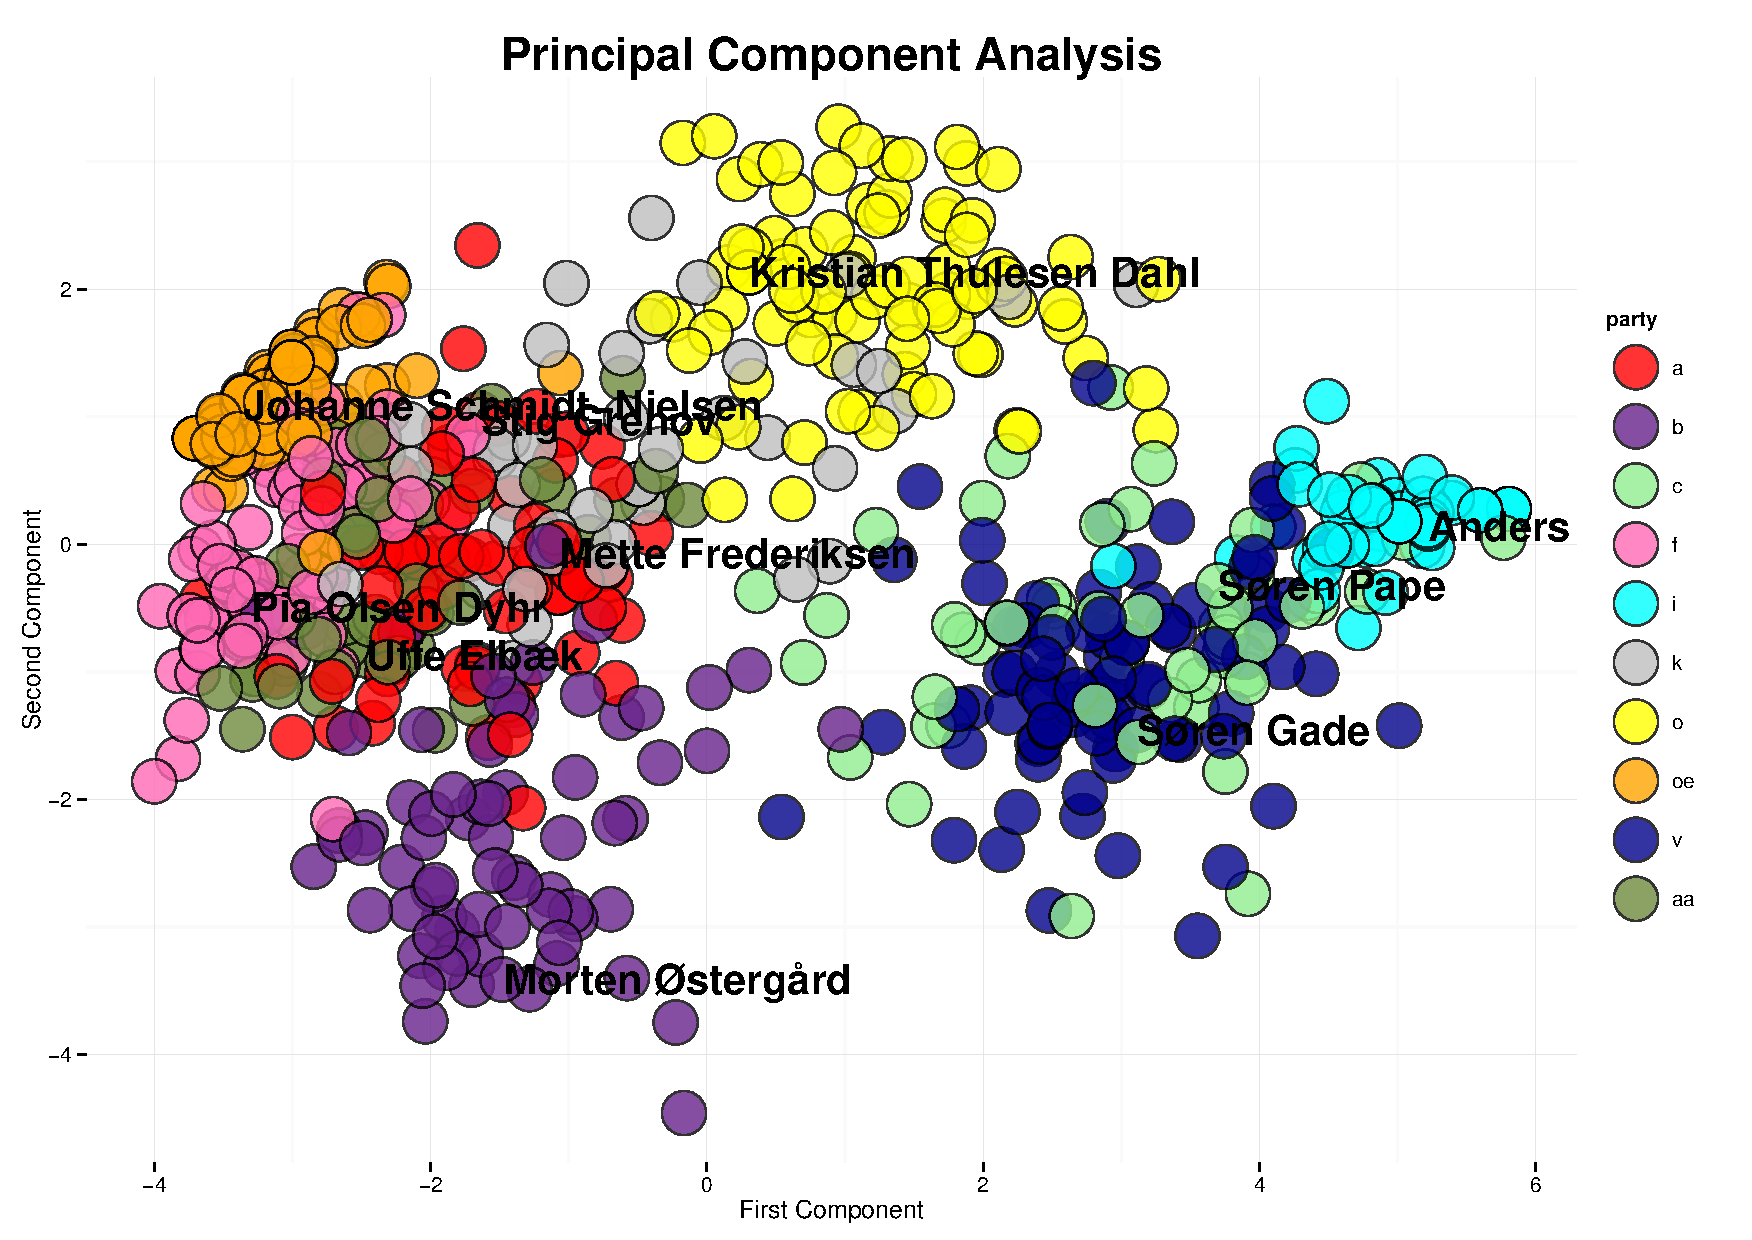
\includegraphics[width=\textwidth]{PCA1}
\end{figure}
The first thing we notice from the PCA plot is that there seems to be a nice grouping of the parties and that a classical left-right scale seems to appear on the horizontal axis (first component). The left wing parties seem to group together to the left, with Enhedslisten clustered together and Socialdemokratiet and Alternativet slightly more spread out. To the right the candidates from Liberal Alliance is also clustered neatly together whereas both Venstre and Konservative are vastly spread out. It is also visually clear that the first component contains the most variance since the vertical axis (second component) mainly contributes with the information that Radikale Venstre and Dansk Folkeparti seemingly are opposed to each other in this dimension. 
As mentioned it seems that the first component, portrayed as the horizontal axis, could be capturing the classical left/right-socialism/liberalism spectrum, driven by distributional politics. Political theory would predict the secondary axis to be driven by value-based politics which makes sense having Radikale and DF opposed to each other - but this does not also explain Enhedslisten and DF supposedly sharing the same values. In fact it seems that the parties that are sharing the same values on the vertical scale usually agree on matters of EU. Let us take a look at the loadings for the first two components to see which variables (questions) are driving  the distribution of the parties in the spectrum plot.
\begin{figure}[H]
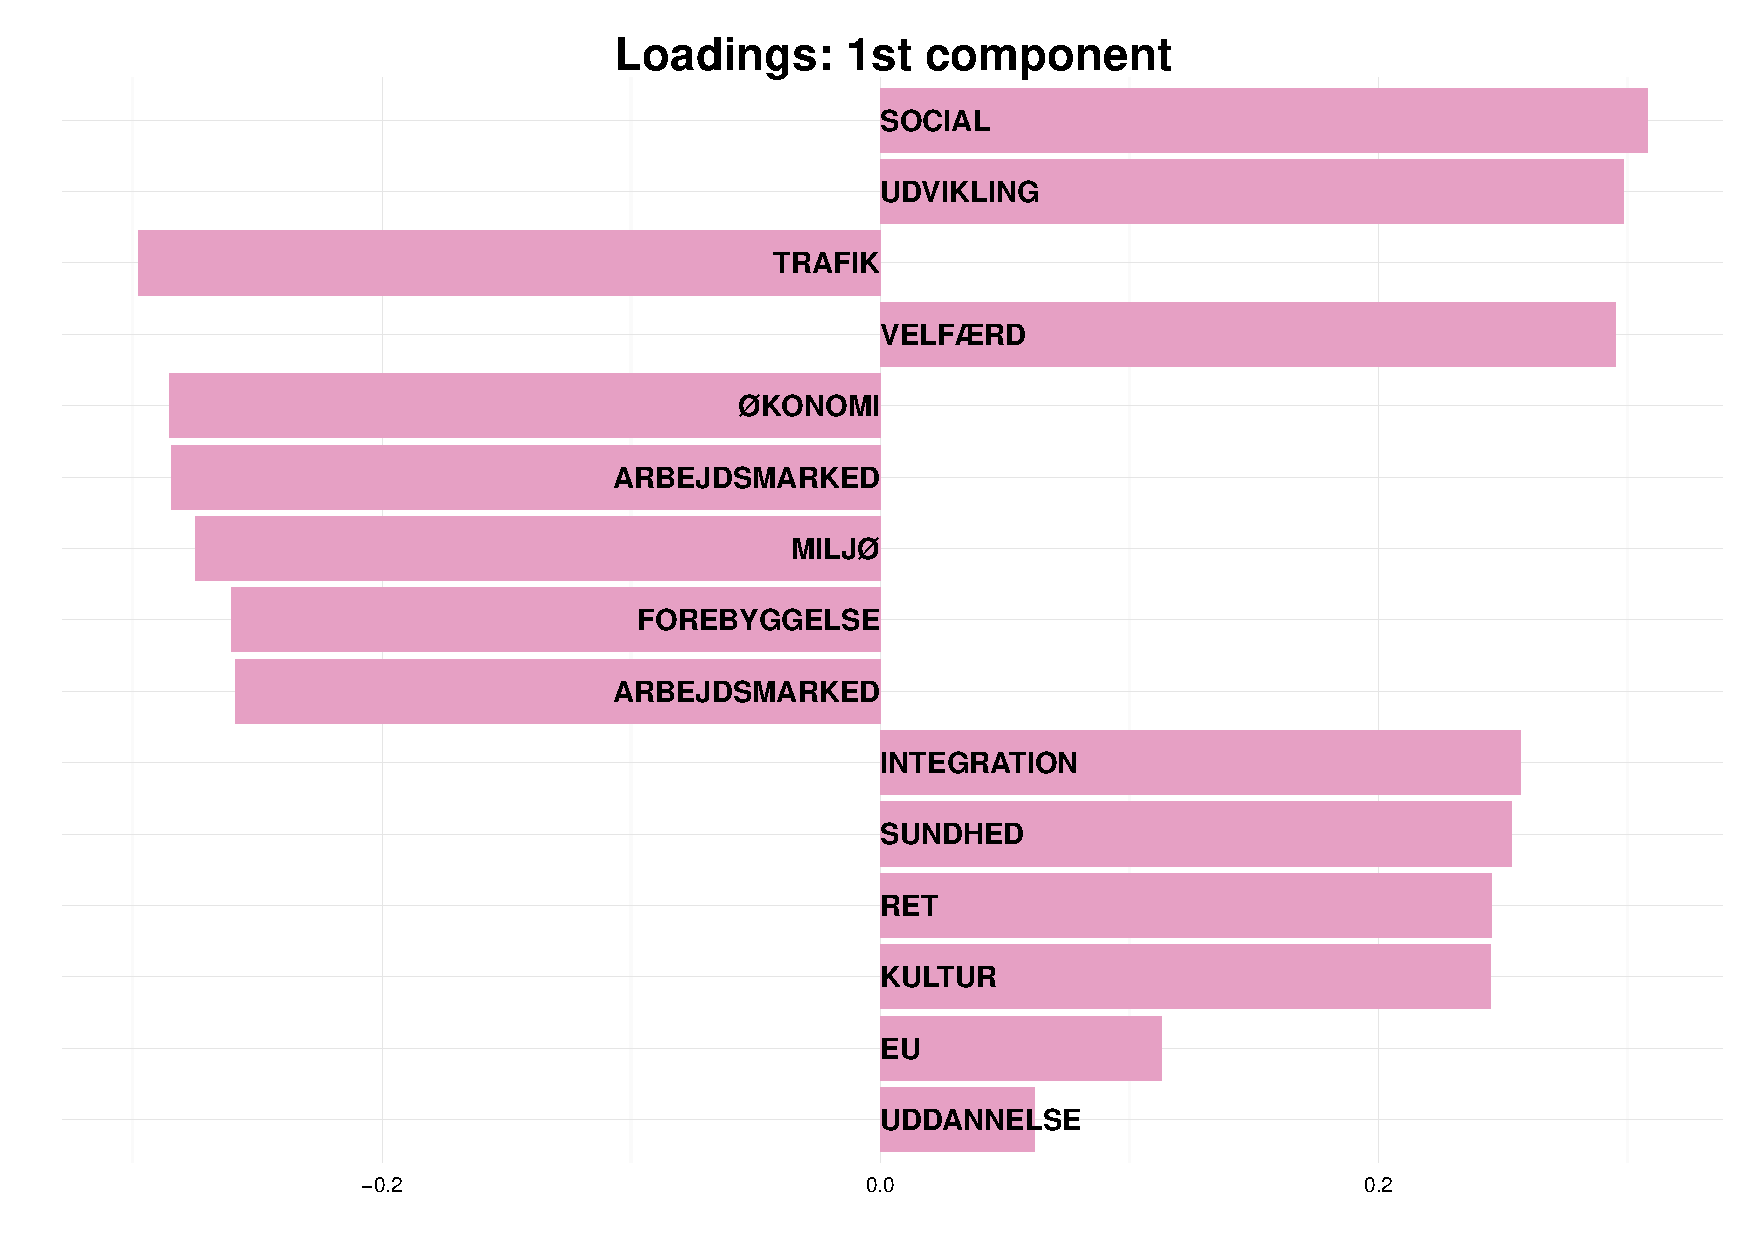
\includegraphics[width=0.5\textwidth]{loadings1}
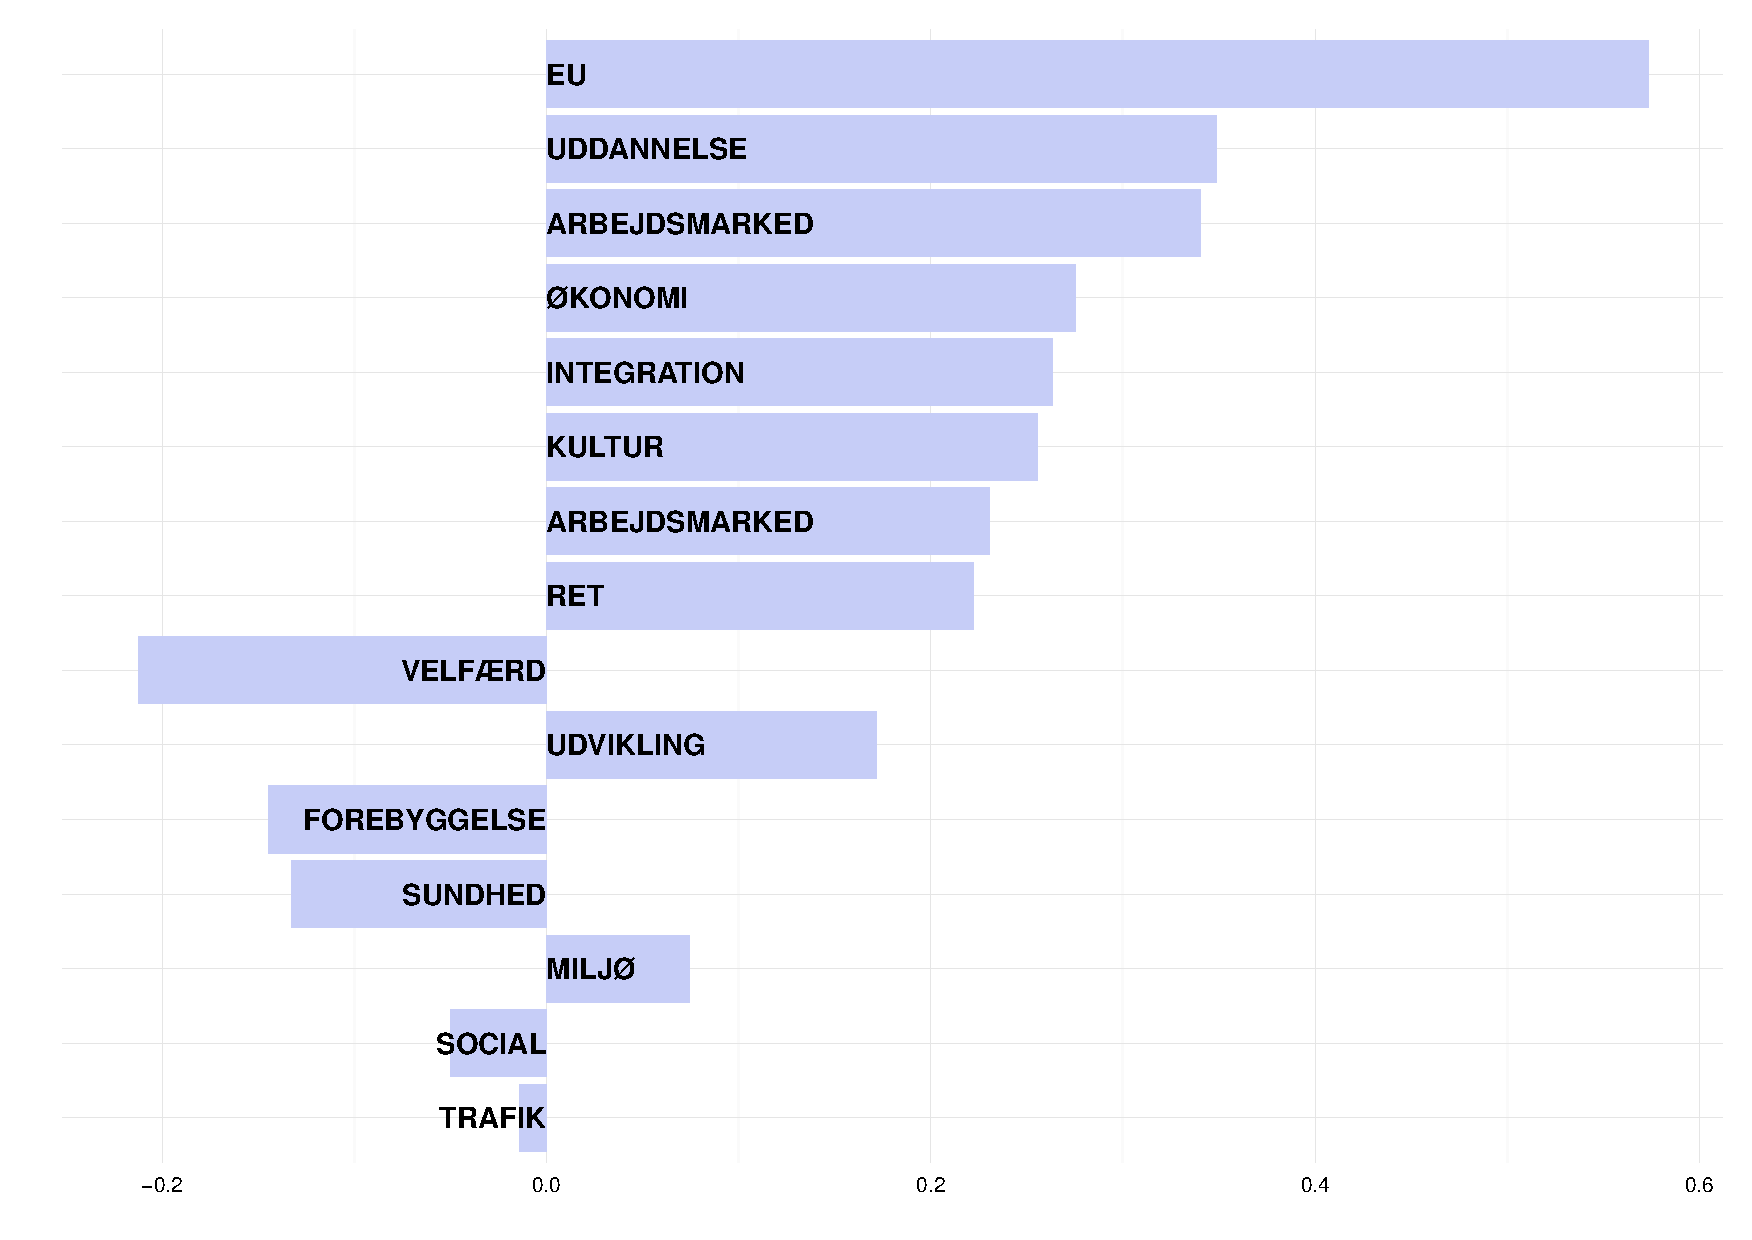
\includegraphics[width=0.5\textwidth]{loadings2}
\end{figure}
The two plots depict the loadings of the first two component in the PCA, ordered according to the loadings’ absolute value. As we see from the left figure, the variation in the first component is mainly driven by questions on welfare benefits, development aid and investments in public transport. As anticipated the loadings of the second component is driven mainly by the question on EU’s role and influence, but also by questions on the public school reform and unemployment benefits. 
A reason why we may not see a crystal clear political spectrum aligned with the political science literature could also be the weighting of the different questions - or rather, the lack thereof. One could argue that a candidate’s views on criminal justice and integration should not weigh as heavily as views on public sector size and levels of unemployment benefits when trying to depict the candidates on a distributional left-right-scale. Vice versa we would want issues on integration and environmental politics to weigh more when plotting the value-based political spectrum. The candidates are not asked to weigh the questions individually (as seen in FINNISH paper, ref.)
Therefore we try and subset our initial dataset into two separate datasets grouped by questions regarding distributional and value-based politics respectively. Questions on distributional politics are statements such as “Growth in the public sector is more important than tax reliefs”, “Unemployment benefits should be lowered, making it more profitable to take a job” and “A visit to the general practitioner should cost 100DKR.”. Questions on value-based politics are statements like “Public institutions are too considerate towards religious minorities” and “EU have too much power over Danish law”. We perform two separate PCAs on these segregated datasets and plot the two first components in the same plot, in order to see if the political spectrum is more visible now.

[Nyt PCA-plot]

Again, we try to plot the distributional political views on the x-axis and the value-based political views on the y axis. Our new plot differs from the original PCA plot in two ways - the parties are more difficult to entangle and there seems to be a strong correlation between the two axes. 
\section{Can we predict the party outcome bases on the VAA questions?}


\section{The political landscape: VAAs and Election outcomes}
The question of whether VAAs have an impact on election outcomes has been discussed extensively in the literature, and is of interest not just for academics, but as a general objective of obtaining a deeper understanding of how democracies work. Given the sheer magnitude of the voters who turn to VAAs (more than 25\% of Danish voters took the DR test), the question becomes even more pressing. Entangling the effects of VAAs has however proven difficult - previous literature mostly relies on methods of surveys; INDSÆT BESKRIVELSER AF TIDLIGERE STUDIER HER.
In this section, we present a new test for the impact of VAAs on election outcomes, that uses only the candidates’ responses to the VAA (as well as some background data). This research should be taken as a preliminary indication of a specific type of impact test, namely testing for the possibilty of ‘gaming the system’, by taking a position that is ‘unoccupied’ by others, rather than a general test for its impact. Nevertheless, we hope our approach can be a valuable addition to the literature in this account. The main hypothesis we attempt to test is the following;
Hypothesis 1:
Candidates that make themselves distinct will receive more personal votes. 
We propose the following reasoning behind the hypothesis: if voters’ preferences map into responses in a sufficiently ‘noisy’ way, a candidate who has a higher ‘distance’ to other candidates, would end up as the top candidate with a higher number of test takers, than candidates who lie very close to others. If VAAs have a discernible impact on voting behavior, candidates who are more likely to end up on top of the results with test takers should receive more personal votes. 
However, an opposite mechanism could be expected to exist: when candidates are observed to cluster around a specific position, we might hypothesize that it such positions would be popular among voters. As above, this would lead candidates in such positions to end up as the top candidate with more test takers, if voters and candidates cluster around the same positions. 
It is important to note, that our identification method does not allow us to explicitly distinguish these two mechanism from one another. A highly robust method of doing so, would likely require data on the test takers’ responses to the VAA. We were unfortunately not able to obtain this data from DR. One way of alleviating this issue is to measure distinctiveness for any candidate, not from the entire set of remaining candidates, but only for those within the same party and the same voting district (storkreds). 
As a graphical representation of the ideas, see FIGURE BELOW. Assume that three candidates, A, B and C are fairly close on political opinions, but there is higher agreement between B and C, than between Candidate A and the two others. If voters responses to a VAA are spread noisily over the depicted policy space, Candidate A will have a larger area to ‘herself’, and will therefore be shown as the top result with more voters. However, if Candidates B and C are clustered around an opinion that is also popular with test takers (and voters) they are likely to receive more personal votes.
[figur - politisk enighed]

\subsection{Measures of distance and distinctiveness of a candidate}
Our identification strategy rests on two primary elements: First, we need a precise definition of the distance between two candidates. Second, we need an appropriate method of capturing the distance measure for each candidate, which requires answering the question: for any one candidate, who are the relevant other candidates to measure the distance to? Both will be elaborated on below.
While the data science toolbox provides a wide array of options for assessing distance between points in multi-dimensional, potentially correlated space (e.g. Euclidean distance, Mahanolobi’s distance) we have chosen a definition that mirrors the assumed mechanism of our hypothesis: the ‘agreement’ measure actually used in computing the results of a VAA. As described in Section 1, users are shown a ‘percentage agreement’ with candidates based on their responses to the VAA. The percentage agreement between Candidate i and Candidate j is defined as,
\begin{equation}
agree.mean_{i}	=	\dfrac{1}{n_{P_{i}}}\cdot\sum_{P_{i}}agree_{i,p}
\end{equation}
where $n_{P_{i}}$ is the number of candidates in the set $P_i$.

\subsection{Identification strategy}
Our identification strategy relies on a linear regression framework using data from the entire sample. Before we proceed with the model, it is worth dwelling shortly on the distinction between this approach and the data scientific approach used above in SECTIONS XX AND XX. MACHINE LEARNING: INFERENS KONTRA PREDICTION.
Our variable of interest is the number of personal votes a candidate receives. As described in SECTION 1  .... The personal votes a candidate receives is the most precise measure of a candidates’ election outcome, and has more variation than the binary election outcome (elected or not). Our baseline regression model is the following,
\begin{equation}
votes_{i}=\beta_{0}+\beta_{1}agree_{i,j}+\boldsymbol{\beta}'\mathbf{X}_{i}+\varepsilon_{i}
\end{equation}
where we are most interested in the estimate of $\beta_{1}$, which measures the impact of being close to other candidates. A negative $\beta_{1}$ implies a positive effect of being ‘distinct’ from other candidates. The variables in $X_{i}$ represent control variables such as background demographic information and whether or not the candidate has previously been elected - they will be included in case there is any covariance with $agree_{i,j}$, which would otherwise imply a biased estimate of $\beta_{1}$.

\section{Conclusion}
[...]


\end{document}